\chapter{处理配分函数}
\label{chap:18}
% Partition Function 配分函数的定义见 wiki:https://www.wikiwand.com/zh/%E9%85%8D%E5%88%86%E5%87%BD%E6%95%B0

%%%%%%%%%%%%%%%%%%%%%%%%%%%%%%%%%%%%%%%%%%%%%%%%%%%%%%%%%
%%%%%%%%%%%%%%%%%%% author:quxiaofeng %%%%%%%%%%%%%%%%%%%
%%%%%%%%%%%%%%%%%%%%%%%%%%%%%%%%%%%%%%%%%%%%%%%%%%%%%%%%%

如 \consider{16.2.2 节}中所见,很多概率模型(一般称为无向图模型)是用\consider{(非正态/未标准化/unnormalized)概率分布 \mbox{ \(\widetilde{p}(\bm{x};\bm{\theta})\)} }定义的。用配分函数\footnote{译者注:配分函数(Partition Function)的定义见 wiki:\url{https://www.wikipedia.org/zh/\%E9\%85\%8D\%E5\%88\%86\%E5\%87\%BD\%E6\%95\%B0}}\(Z(\bm{\theta})\)去除\(\widetilde{p}\)来得到一个概率分布:
\begin{equation}
    p(\bm{x};\bm{\theta})
    = \frac{1}{Z(\bm{\theta})}\widetilde{p}(\bm{x};\bm{\theta}).
\end{equation}

配分函数是\consider{非标准化}概率对于所有状态的积分(连续变量)或和(离散变量): 
\begin{equation}
    \int\widetilde{p}(\bm{x})d\bm{x}
\end{equation}
 或者
 \begin{equation}
     \sum_{\bm{x}}\widetilde{p}(\bm{x}).
 \end{equation}

这个运算对于很多常用模型来说是\consider{不可解的(intractable)}。

如\consider{20 章}所见,有些深度学习模型在设计上是有可解标准化常量的,或者无需计算\(p(\bm{x})\)。但其它的模型就需要直接面对不可解配分函数的问题了。本章我们讨论训练和评估具有不可解配分函数的模型的方法。

\section{对数似然梯度}
\label{sec:18.1}

使用最大似然法学习无向模型的难点在于配分函数有参数依赖。相对参数的对数似然梯度具有与配分函数梯度相关项:
\begin{equation}
    \nabla_{\bm{\theta}}\log{p(\bm{x};\bm{\theta})}
    = \nabla_{\bm{\theta}}\log{\widetilde{p}(\bm{x};\bm{\theta})}
    - \nabla_{\bm{\theta}}\log{Z(\bm{\theta})}.
\end{equation}

这里就是著名的\consider{正相(positive phase)学习与负相(negative phase)学习}分解的产生。

对于大多数我们所关心的无向图模型,负相比较难。没有隐变量或者隐变量\consider{交互,连接}比较少的模型一般具有可解的正相。具有简单正相、复杂负相的模型的最基础的例子就是 RBM。给定可见单元,RBM 的隐单元之间条件独立。正相复杂、隐变量之间交互复杂的例子,主要集中于第 19 章。本章关注负相的复杂度。

再仔细观察一下\(\log Z\)的梯度:
\begin{align}
    & \nabla_\theta \log{Z}                                \\
    & = \frac{\nabla_\theta Z}{Z}                          \\
    & = \frac{\nabla_\theta\sum_x\widetilde{p}(\bm{x})}{Z} \\
    & = \frac{\sum_x\nabla_\theta\widetilde{p}(\bm{x})}{Z}.
\end{align}

若模型对所有 \(\bm{x}\) 都有 \(p(\bm{x})>0\),则可用 \(exp(\log\widetilde{p}(\bm{x}))\) 代换 \(\widetilde{p}(\bm{x})\):
\begin{align}
& \frac{\sum_x\nabla_\theta\exp(
	\log{\widetilde{p}(\bm{x})})}{Z}             \\
& = \frac{\sum_x\exp(\log{\widetilde{p}(\bm{x})})
	\nabla_\theta\log{\widetilde{p}(\bm{x})}}{Z} \\
& = \frac{\sum_x\widetilde{p}(\bm{x})
	\nabla_\theta\log\widetilde{p}(\bm{x})}{Z}   \\
& = \sum_{\bm{x}}p(\bm{x})
	\nabla_\theta\log\widetilde{p}(\bm{x})       \\
& = \mathbb{E}_{x\sim{}p(\bm{x})}
	\nabla_\theta\log\widetilde{p}(\bm{x}).
\end{align}

这个推导利用了离散 \(\bm{x}\) 的求和。对于连续的 \(\bm{x}\),利用积分也可以得到相似的结果。在连续版的推导中,可以使用积分号下的莱布尼茨法则得到同样的结果
\begin{equation}
    \nabla_{\bm{\theta}}\int\widetilde{p}(\bm{x})d\bm{x}
    = \int\nabla_{\bm\theta}\widetilde{p}(\bm{x})d\bm{x}.
\end{equation}
这一等同的结果只是在 \( \widetilde{p} \) 和 \( \nabla_{\bm\theta}\widetilde{p}(\bm{x})d\bm{x} \) 满足一定的正则化条件时成立。根据测度论,需要满足如下条件:(i) 非正态分布\( \widetilde{p} \) 对任意 \(\bm{\theta}\)都是 \(\bm{x}\) 的勒贝格可积函数;

\begin{equation}
    \nabla_{\bm{x}}\log{}Z
    = \mathbb{E}_{\bm{x}\sim{}p(\bm{x})}
    \nabla_{\bm{\theta}}\log\widetilde{p}(\bm{x})
\end{equation}

\section{随机最大似然和对比分歧}
\label{sec:18.2}

\begin{algorithm}
\DontPrintSemicolon
设置 \(\epsilon\),步长,应设为较小正数。\;
设置 \(k\),吉布斯(Gibbs)步长,为一个较大的值,为预热(burn in)提供冗余。在一个小图像块上训练 RBM 大约可以设为 100。\;
\While{未收敛}{
    从训练集中抽样一个包含 \(m\) 个样本 \(\{\bm{x}^{(1)},\ldots,\bm{x}^{(m)}\}\) 的小批(minibatch)\;
    \(\bm{g} \longleftarrow \frac{1}{m}\sum^m_{i=1}
    	\nabla_{\bm{\theta}}\log\widetilde{p}(\bm{x}^{(i)};\bm{\theta})\).\;
    用随机数初始化一组 \(m\) 个样本(可以使用例如均匀分布或正态分布,或者也可以使用与目标边缘分布想匹配的分布)。\;
    \For{\(i=1\) to \(k\)}{
    	\For{\(i=1\) to \(k\)}{
        	\(\widetilde{\bm{x}}^{(j)} 
            \longleftarrow \text{吉布斯更新}(\widetilde{\bm{x}}^{(j)}).\)\;
        }
    }
    \(\bm{g} \longleftarrow
    	\bm{g} - \frac{1}{m}\sum^m_{i=1}
    	\nabla_{\bm{\theta}}\log\widetilde{p}(\bm{x}^{(i)};\bm{\theta})\).\;
    \(\bm{\theta} \longleftarrow
    	\bm{\theta} + \epsilon\bm{g}\)\;
}
\caption{一个简单的蒙特卡洛马尔科夫链算法(MCMC)算法。利用梯度上升来计算带有可解配分函数的对数似然\label{alg:18.1}}
\end{algorithm}

\begin{figure}[htbp] %  figure placement: here, top, bottom, or page
   \centering
   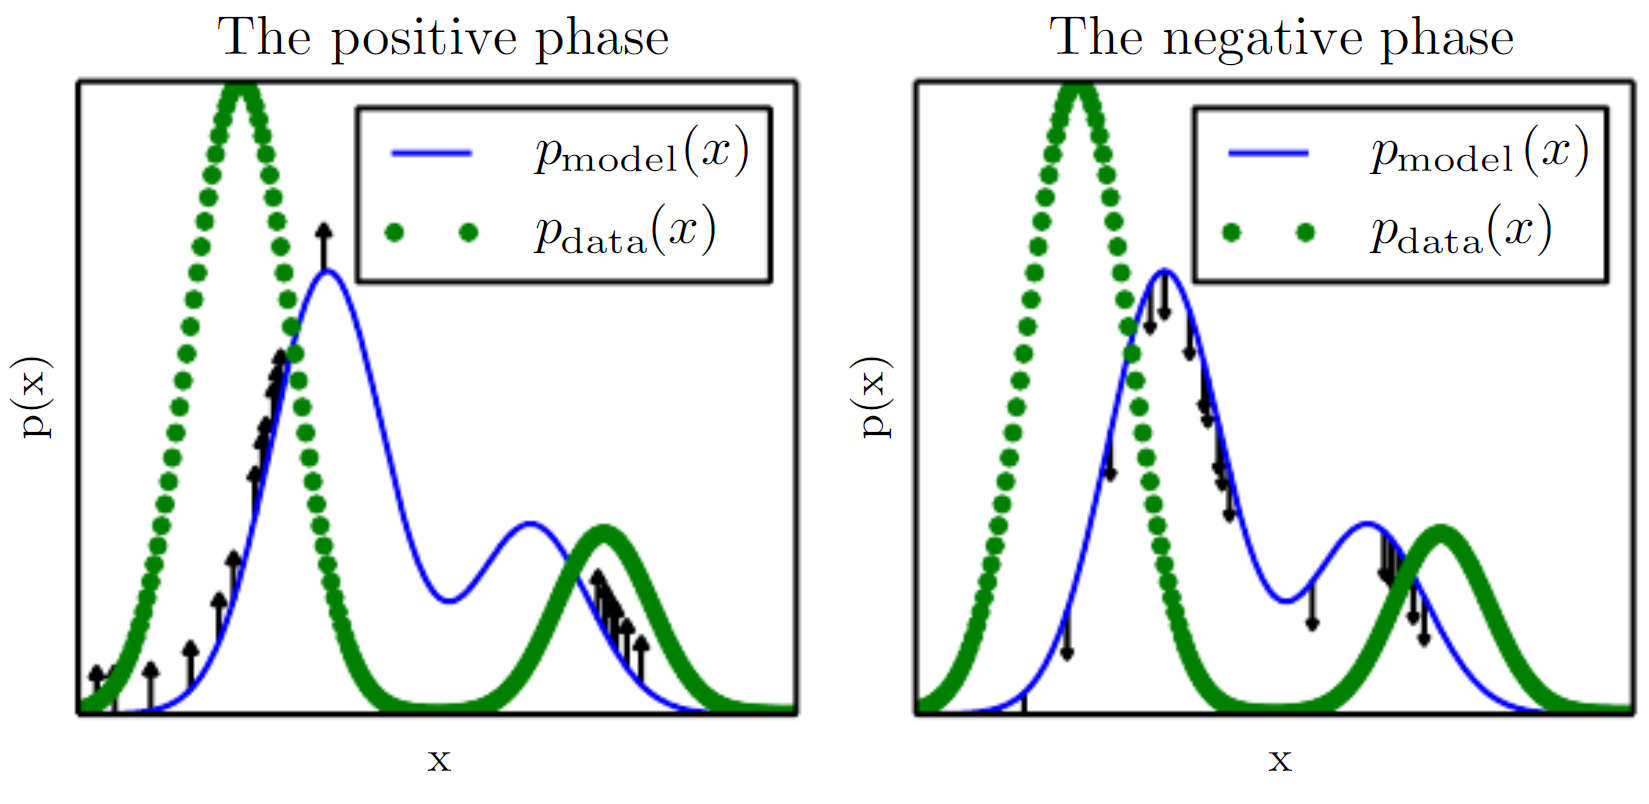
\includegraphics[width=\textwidth]{fig/chap18/18_1.png} 
   \caption{算法 18.1 的``正相''和``负相''}
   \label{fig:18.1}
\end{figure}

\begin{algorithm}
\DontPrintSemicolon
设置 \(\epsilon\),步长,应设为较小正数。\;
设置 \(k\),吉布斯(Gibbs)步长,为一个较大的值,为预热(burn in)提供冗余。在一个小图像块上训练 RBM 大约可以设为 100。\;
\While{未收敛}{
    从训练集中抽样一个包含 \(m\) 个样本 \(\{\bm{x}^{(1)},\ldots,\bm{x}^{(m)}\}\) 的小批(minibatch)\;
    \(\bm{g} \longleftarrow \frac{1}{m}\sum^m_{i=1}
    	\nabla_{\bm{\theta}}\log\widetilde{p}(\bm{x}^{(i)};\bm{\theta})\).\;
    用随机数初始化一组 \(m\) 个样本(可以使用例如均匀分布或正态分布,或者也可以使用与目标边缘分布想匹配的分布)。\;
    \For{\(i=1\) to \(k\)}{
    	\For{\(i=1\) to \(k\)}{
        	\(\widetilde{\bm{x}}^{(j)} 
            \longleftarrow \text{吉布斯更新}(\widetilde{\bm{x}}^{(j)}).\)\;
        }
    }
    \(\bm{g} \longleftarrow
    	\bm{g} - \frac{1}{m}\sum^m_{i=1}
    	\nabla_{\bm{\theta}}\log\widetilde{p}(\bm{x}^{(i)};\bm{\theta})\).\;
    \(\bm{\theta} \longleftarrow
    	\bm{\theta} + \epsilon\bm{g}\)\;
}
\caption{对比分歧算法。用梯度上升优化\label{alg:18.2}}
\end{algorithm}

\begin{figure}[htbp] %  figure placement: here, top, bottom, or page
   \centering
   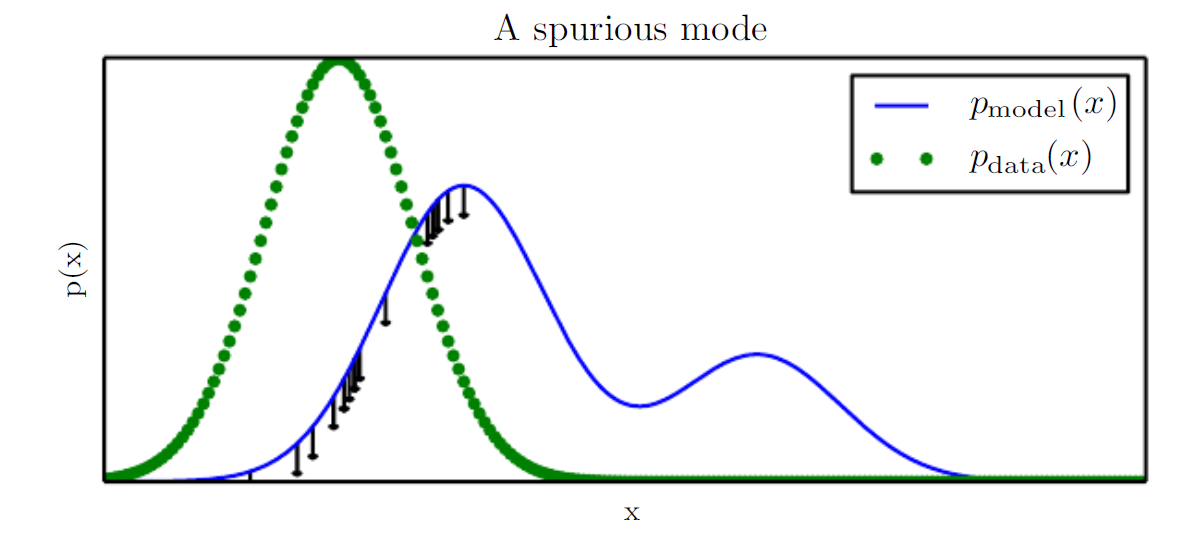
\includegraphics[width=\textwidth]{fig/chap18/18_2.png} 
   \caption{对比分歧的负相(根据算法 18.2)}
   \label{fig:18.2}
\end{figure}

\section{伪概率}
\label{sec:18.3}

\section{评分比对和比率比对}
\label{sec:18.4}

\section{评分比对的降噪}
\label{sec:18.5}

\section{噪声抑制期望}
\label{sec:18.6}

\section{配分函数期望}
\label{sec:18.7}

\subsection{基于退火算法的重要性采样}
\label{sec:18.7.1}

\subsection{桥采样}
\label{sec:18.7.2}